\documentclass[letterpaper,10pt,conference]{ieeeconf}

\IEEEoverridecommandlockouts
\overrideIEEEmargins

\usepackage{amsmath}
\usepackage{amssymb}
\usepackage{booktabs}
\usepackage{cite}
\usepackage{graphicx}
\usepackage{url}

\title{\LARGE \bf
STRIDE: Safe Task-Return and Intent-Driven Execution for Humanoid Vision-Language Navigation}

\author{Anonymous Authors}

\begin{document}
\maketitle
\thispagestyle{empty}
\pagestyle{empty}

\begin{abstract}
Vision-language navigation (VLN) policies can select semantically meaningful actions, but a humanoid executor also needs to reject unsafe motions, recover without losing the task intent, and stop at the right time. This paper presents STRIDE, an execution wrapper for humanoid VLN that couples intent tracking, safety gating, stop verification, and task-return recovery. STRIDE does not replace the language-conditioned policy; it mediates each proposed motion skill through a safety and progress layer, and when a motion is rejected it executes a local recovery sequence that attempts to return to the same task intent rather than terminating or drifting into open-loop avoidance. In a locked local evaluation with 50 held-out episodes per method, STRIDE reaches 30/50 safe successes with zero unsafe violations. Three external adapted baselines each reach 18/50 safe successes with zero unsafe violations in the same evaluation. Ablations indicate that stop verification and task-return replan are the components most associated with the observed safe-success difference. All reported table values are generated from local CSV/JSON artifacts and checked by an accompanying consistency script.
\end{abstract}

\section{Introduction}
Vision-and-language navigation asks an embodied agent to follow natural-language instructions from egocentric observations~\cite{anderson2018r2r}. Recent video-based and legged-robot VLN systems show that learned policies can produce useful next-step actions from visual history and instruction context~\cite{zhang2024navid,cheng2024navila}. For humanoid robots, however, high-level semantic correctness is not enough. A candidate action must be executable by a whole-body controller, must avoid unsafe contact, and must preserve the user intent after local recovery.

The central failure mode studied here is not simply collision. A conservative safety filter can avoid unsafe actions but repeatedly reject forward progress until the episode times out. Conversely, a purely task-driven policy can keep pursuing the instruction while crossing unsafe regions. STRIDE targets the intermediate regime: reject unsafe motions, perform a local recovery, reacquire the visual goal when possible, and return to the original navigation task.

This draft makes three narrow contributions. First, it describes STRIDE as an intent-preserving execution layer for humanoid VLN. Second, it defines a locked local evaluation protocol with adapted baselines from MPC-CBF~\cite{zeng2021mpccbf}, SafeDPA~\cite{xiao2023safedpa}, and SPARK-style runtime safety filtering~\cite{sun2025spark}; these are adapted baselines, not official reproductions. Third, it reports generated tables and vector figures whose numeric values are checked against local artifacts.

The scope is intentionally limited. The results are a paper-draft summary of existing artifacts, not a new experimental run. We do not claim hardware deployment, official baseline reproduction, or superiority beyond the logged evaluation setting.

\section{Problem Setting and Metrics}
The evaluation considers language-conditioned humanoid navigation episodes. At each step, a visual-language policy proposes a discrete motion skill, such as moving forward, turning, backing off, or stopping. An execution layer can accept the proposal, reject it, replace it with a recovery action, or verify a stop. The low-level whole-body execution stack follows the local motion command; the paper focuses on the decision layer above that stack.

Let an episode be a sequence of observations $o_t$, instruction context $x$, policy proposals $a_t$, and executed skills $u_t$. STRIDE maintains an internal intent state $z_t$ that summarizes the current instruction target, recent visual evidence, and whether the previous policy proposal was blocked. The wrapper chooses
\begin{equation}
    u_t = \pi_{\mathrm{exec}}(a_t, o_t, x, z_t),
\end{equation}
where $\pi_{\mathrm{exec}}$ is constrained by the safety gate and the stop verifier.

We report five metrics. Safe success is task success without any evaluator-reported unsafe violation. Unsafe is the number and rate of unsafe violations. Timeout is the number and rate of episodes that reach the step limit without success. Intervention rate is the fraction of executed steps where the safety or recovery layer intervenes. Mean final distance is the final-distance summary emitted by the local evaluator. These metrics are intentionally compact because every number in the result tables is read from CSV/JSON artifacts.

\section{STRIDE}
Fig.~\ref{fig:overview} summarizes the execution loop. STRIDE is built around four components: intent state tracking, safety gating, stop verification, and task-return recovery.

\begin{figure*}[t]
  \centering
  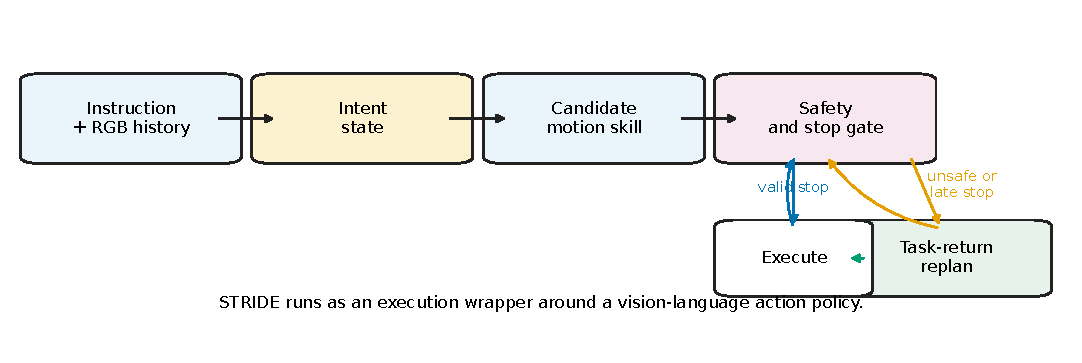
\includegraphics[width=0.98\textwidth]{figures/stride_overview.pdf}
  \caption{STRIDE overview. This is a generated schematic, not a camera frame. A language-conditioned policy proposes a motion skill; STRIDE checks safety and stop validity, then either executes the skill or runs task-return recovery.}
  \label{fig:overview}
\end{figure*}

\subsection{Intent State}
The intent state is a short-horizon memory of what the policy appears to be pursuing. It is not an oracle goal and does not use privileged success, shortest-path, or waypoint information during execution. Instead, it stores the recent instruction-conditioned visual context, whether the target evidence was retained or reacquired, and whether a recovery sequence has recently unblocked forward progress.

This state matters because a humanoid recovery action can be locally valid but semantically harmful. For example, a turn or backoff may clear an obstacle, but after that detour the policy should continue toward the same instruction target, not simply maximize free space. STRIDE therefore treats recovery as a temporary deviation from the task, followed by an explicit return to policy-driven navigation.

\subsection{Safety Gate}
The safety gate evaluates each proposed skill before execution. If the candidate is accepted, it is passed to the low-level controller. If it is rejected, the gate records the blocked proposal and activates recovery. The gate is deliberately conservative: unsafe candidates should not be executed merely because they might make semantic progress.

This design creates a second problem: a conservative gate can induce repeated rejection loops. STRIDE addresses that loop with task-return recovery rather than with a terminal stop. The recovery module selects bounded local skills such as small turns, backoff, or open-space seeking, then returns control to the policy once the local state is unblocked.

\subsection{Stop Verification}
VLN policies often emit stop when the visual-language context suggests that the target has been reached. In embodied execution, premature stop and late stop are both costly. STRIDE adds a stop verifier that checks whether a proposed stop is consistent with recent intent evidence and local progress. A rejected stop is treated as a recoverable action mismatch rather than as a terminal failure.

The verifier is not an oracle success checker. It is a local consistency check over the same execution-time context used by the wrapper. In the locked artifacts, removing this verifier lowers safe success from 30/50 to 23/50 while preserving zero unsafe violations, as shown in Table~\ref{tab:ablation}.

\subsection{Task-Return Recovery}
Fig.~\ref{fig:task_return} illustrates the recovery behavior. When the current candidate is blocked, STRIDE runs a bounded recovery sequence and then re-enters the policy loop with the same instruction intent. This differs from a pure local safety filter: the goal is not only to avoid the immediate unsafe motion, but to make the next policy action useful again.

\begin{figure*}[t]
  \centering
  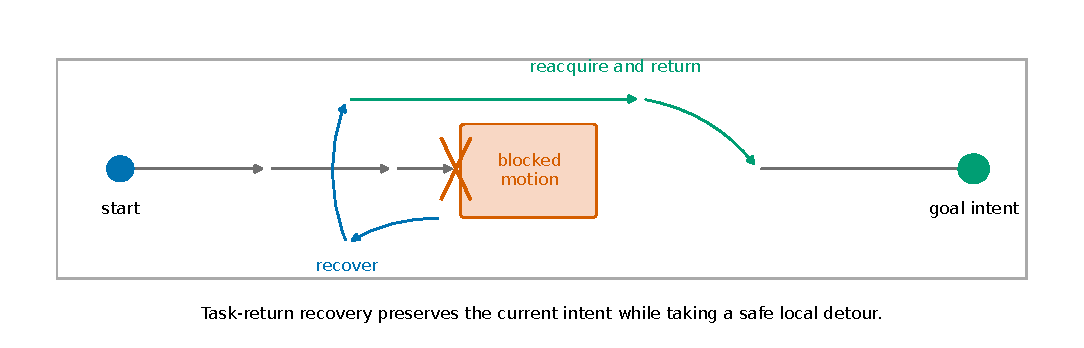
\includegraphics[width=0.98\textwidth]{figures/task_return_recovery.pdf}
  \caption{Task-return recovery schematic. The blocked motion is rejected, a local detour is executed, and control returns to the same instruction intent. This is a generated schematic, not a camera frame.}
  \label{fig:task_return}
\end{figure*}

\section{Experimental Protocol}
The reported numbers come from local locked artifacts. Each method is evaluated on 50 held-out episodes with the same language tasks, split, unsafe evaluator, and success evaluator. The maximum episode length is 180 steps. Large logs, videos, and frames remain outside the git-tracked paper directory; this draft uses only lightweight CSV/JSON summaries.

STRIDE is compared against three adapted baselines. MPC-CBF humanoid adapted follows the model-predictive control and control-barrier-function safety-filter family~\cite{zeng2021mpccbf}. SafeDPA adapted follows the idea of safe policy adaptation with a control-barrier safety layer~\cite{xiao2023safedpa}. SPARK-style adapted follows the runtime humanoid safety-filtering style of SPARK~\cite{sun2025spark}. These are adapted baselines for the local humanoid VLN harness, not official reproductions of the original systems.

The humanoid execution setting builds on a whole-body motion-control stack in the style of recent humanoid tracking systems~\cite{luo2025sonic}. The policy side is a video-conditioned VLN executor, motivated by recent visual-language navigation models~\cite{zhang2024navid}. The evaluation here isolates the safety and recovery wrapper rather than retraining the underlying policy.

\section{Results}
Table~\ref{tab:main_comparison} gives the main locked comparison. STRIDE achieves 30/50 safe successes with zero unsafe violations. The three adapted baselines each achieve 18/50 safe successes with zero unsafe violations. Thus, in this artifact set, the difference is not unsafe-rate reduction among the adapted safety methods; all four safety-aware rows report zero unsafe violations. The difference is task completion under the same safety constraint.


\begin{table}[t]
\caption{Main locked comparison. External methods are adapted baselines, not official reproductions.}
\label{tab:main_comparison}
\centering
\scriptsize
\setlength{\tabcolsep}{1.7pt}
\begin{tabular}{@{}lcccc@{}}
\hline
Method & Type & Safe & Unsafe & Dist. \\
\hline
\shortstack[l]{STRIDE} & proposed method & 30/50 (0.60) & 0 (0.00) & 3.06 \\
\shortstack[l]{MPC-CBF humanoid\\adapted} & adapted baseline & 18/50 (0.36) & 0 (0.00) & 5.16 \\
\shortstack[l]{SafeDPA\\adapted} & adapted baseline & 18/50 (0.36) & 0 (0.00) & 5.54 \\
\shortstack[l]{SPARK-style\\adapted} & adapted baseline & 18/50 (0.36) & 0 (0.00) & 5.41 \\
\hline
\end{tabular}
\end{table}


The compact metrics in Table~\ref{tab:compact_metrics} show the same pattern with timeout and intervention rates included. STRIDE times out in 19/50 episodes, while each adapted baseline times out in 32/50 episodes. STRIDE also has the lowest intervention rate among these rows. We interpret this cautiously: lower intervention is useful only when paired with zero unsafe violations, and this paper does not claim the same ordering outside the locked setting.


\begin{table}[t]
\caption{Compact metrics table. Intervention rate is per executed step.}
\label{tab:compact_metrics}
\centering
\scriptsize
\setlength{\tabcolsep}{1.45pt}
\begin{tabular}{@{}lccccc@{}}
\hline
Method & Safe & Unsafe & Timeout & Interv. & Dist. \\
\hline
\shortstack[l]{STRIDE} & 30/50 (0.60) & 0 (0.00) & 19 (0.38) & 0.279 & 3.06 \\
\shortstack[l]{MPC-CBF humanoid\\adapted} & 18/50 (0.36) & 0 (0.00) & 32 (0.64) & 0.691 & 5.16 \\
\shortstack[l]{SafeDPA\\adapted} & 18/50 (0.36) & 0 (0.00) & 32 (0.64) & 0.784 & 5.54 \\
\shortstack[l]{SPARK-style\\adapted} & 18/50 (0.36) & 0 (0.00) & 32 (0.64) & 0.710 & 5.41 \\
\hline
\end{tabular}
\end{table}


\begin{figure}[t]
  \centering
  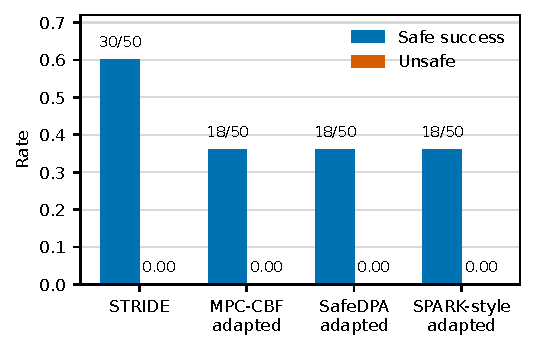
\includegraphics[width=\columnwidth]{figures/results_bar.pdf}
  \caption{Safe-success and unsafe rates from the locked comparison. Values are generated directly from the artifact CSV files.}
  \label{fig:results_bar}
\end{figure}

The ablation in Table~\ref{tab:ablation} separates the components. Removing stop verification reduces safe success to 23/50 and raises the late-stop rate to 0.08. Removing task-return replan reduces safe success to 18/50, matching the adapted baseline safe-success level in this artifact set. Removing late-stop recovery or the visual goal tracker leaves safe success at 30/50 in this run, although the auxiliary stop and distance metrics shift. These results suggest that the strongest observed contributors are stop verification and task-return replan.


\begin{table}[t]
\caption{Ablation on STRIDE components.}
\label{tab:ablation}
\centering
\scriptsize
\setlength{\tabcolsep}{1.45pt}
\begin{tabular}{@{}lccccc@{}}
\hline
Variant & Safe & Unsafe & Stop & Late & Dist. \\
\hline
\shortstack[l]{Full STRIDE} & 30/50 (0.60) & 0 (0.00) & 1.00 & 0.00 & 3.06 \\
\shortstack[l]{w/o stop\\verifier} & 23/50 (0.46) & 0 (0.00) & 0.85 & 0.08 & 4.26 \\
\shortstack[l]{w/o late-stop\\recovery} & 30/50 (0.60) & 0 (0.00) & 0.97 & 0.02 & 3.17 \\
\shortstack[l]{w/o visual goal\\tracker} & 30/50 (0.60) & 0 (0.00) & 1.00 & 0.00 & 3.46 \\
\shortstack[l]{w/o task-return\\replan} & 18/50 (0.36) & 0 (0.00) & 1.00 & 0.00 & 5.20 \\
\hline
\end{tabular}
\end{table}


\begin{figure}[t]
  \centering
  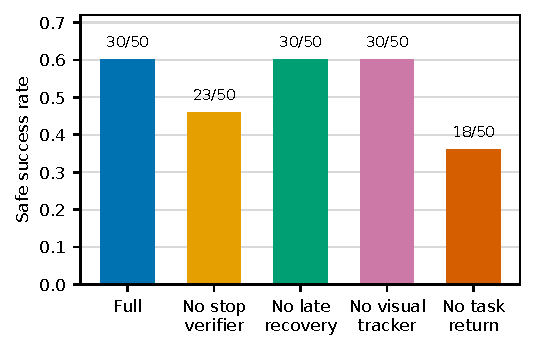
\includegraphics[width=\columnwidth]{figures/ablation_bar.pdf}
  \caption{Ablation safe-success rates. Labels show safe-success counts out of 50 episodes.}
  \label{fig:ablation_bar}
\end{figure}

\section{Discussion}
The main lesson from the artifacts is that safety alone is not the bottleneck after a conservative filter is installed. The adapted baselines all avoid unsafe violations, but their safe-success rates remain lower because they more often fail to complete the task before timeout. STRIDE tries to close that gap by treating rejection as a temporary task interruption, then explicitly returning to the instruction-conditioned policy.

The result should not be overread. The run count is modest, the evaluation is local, and the adapted baselines are not official reproductions. The figures are generated schematics and plots, not real screenshots. The paper also does not establish formal safety guarantees; it reports evaluator-observed unsafe counts. These limitations are important for a submission-quality version and motivate broader held-out splits, official baseline support where possible, and hardware validation.

\section{Conclusion}
STRIDE is an intent-driven execution wrapper for humanoid VLN. In the locked local artifact set, it preserves zero unsafe violations while improving safe success relative to three adapted safety baselines. The ablation points to stop verification and task-return replan as the most important components in this run. The accompanying paper artifacts include generated vector figures, generated tables, source provenance, reviewer notes, and a table consistency check so that numeric claims can be traced back to CSV/JSON files.

\bibliographystyle{IEEEtran}
\bibliography{refs}

\end{document}
